\documentclass[../main.tex]{subfiles}

\begin{document}

\renewcommand{\labelitemi}{\ding{226}}
\renewcommand{\labelitemii}{\ding{227}}

\part{ND280 upgrade}
\label{pt:up}

\chapter{Introduction}
\label{ch:up:motif}
As mentioned in \autoref{ch:T2K:general}, the first goal of the T2K experiment was to measure the $\theta_{13}$ mixing angle. The non-zero value of this angle would open a road towards the CP--violation in the neutrino oscillations. After the successful discovery of the $\theta_{13}$, T2K entered a phase of the precise measurement of the neutrino oscillation parameters. The experiment provides the most precise estimations for the $\theta_{23}$ angle and also very accurate measurements of the $\Delta m_{23}$ and $\theta_{13}$ parameters. Great progress was obtained in the search for the CP--violation with the determination of the 3$\sigma$ confidence level on the possible values of the $\delta_{CP}$~\cite{Abe2020n}. The $\delta_{CP}$ measurement became the main goal of the experiment.

The next-generation experiments like DUNE~\cite{Acciarri2016} and Hyper-Kamiokande~\cite{Proto-Collaboration2018} will be able to achieve 3$\sigma$ sensitivity to the CP--violation across the wide range of the $\delta_{CP}$ values but on the time scale 2026 and beyond. The T2K experiment can probe this effect with less sensitivity but much earlier. The sensitivity of the T2K experiment with the total statistics of $20\times10^{21}$ POT is shown in \autoref{fig:up:sens}.

\begin{figure}[!ht]
  \centering
  \begin{minipage}{0.49\linewidth}
    \centering
    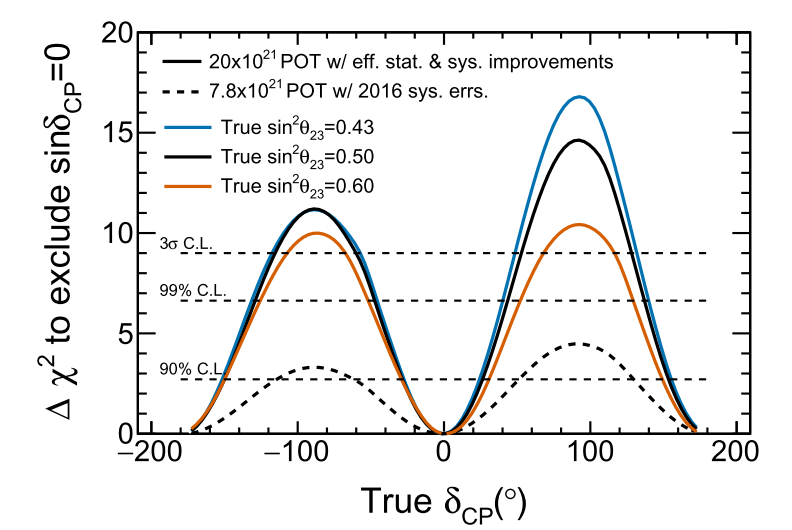
\includegraphics[width = \linewidth]{t2kII_dcp} \\ (a)
  \end{minipage}
  \begin{minipage}{0.49\linewidth}
    \centering
    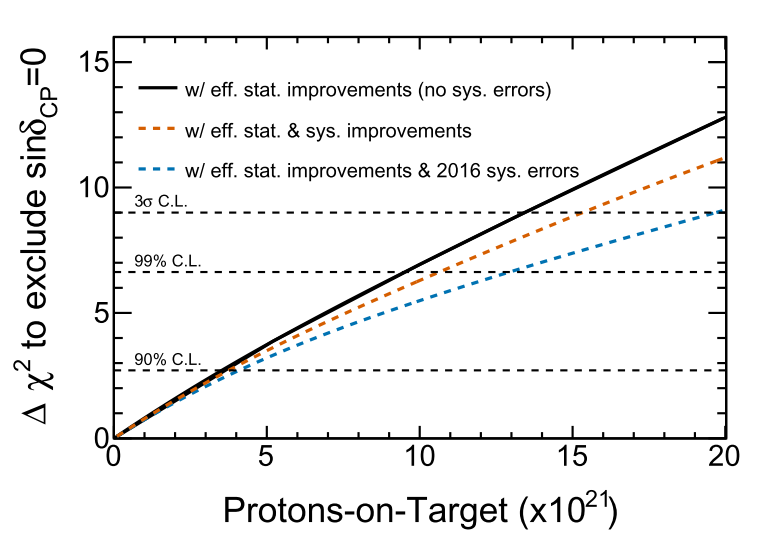
\includegraphics[width = \linewidth]{t2k_cp} \\ (b)
  \end{minipage}
    \caption{An expected sensitivity of the T2K experiment to the CP--violation in the neutrino oscillations. The known mass order is assumed. Three systematic uncertainties estimations are used: (blue) 2016 value, (orange) with improvements by factor 2/3 and (black) only stat. uncertainties. (a) shows the sensitivity over the $\delta_{CP}$ value and (b) shows the sensitivity evolution over the collected statistics for $\delta_{CP}=-\pi/2$.}
    \label{fig:up:sens}
\end{figure}


More statistics is necessary to determine the CP--violation more precisely and to justify if the effect takes place. The improvement of the sensitivity versus the collected data is shown in \autoref{fig:up:sens} b. Initially, the T2K was supposed to collect the total statistics of $7.8\times10^{21}$ POT. The extended run of the T2K experiment aiming at the total statistics $20\times20^{21}$ POT was proposed~\cite{Abe2016e}. This additional period of data collection was called T2K-II. The beamline will be upgraded to provide a more intense neutrino beam (\autoref{sec:up:beam}). Thus the data statistics accumulation will go faster.

There is a room for further improvement of the sensitivity with the reduction of the systematic uncertainty. \autoref{fig:up:sens} presents the sensitivity of the T2K experiment with different assumptions: current systematic uncertainties (in blue), improved systematics by factor 2/3 (in orange), only statistical uncertainty (in black). With the improved systematics, the desired sensitivity will be reached faster, and finally, the wider range of the $\delta_{CP}$ could be studied. The budget of the systematic uncertainties of the T2K experiment is described in~\cite{Abe2017}. The main sources in decreasing order are neutrino cross-sections, flux, secondary interactions in the SK, SK detector. The systematics related to the SK is very hard to reduce and it is going to be extremely expensive. Also, it gives a minor impact. The systematic uncertainty related to the neutrino cross-section and flux could be better constrained with the upgrade of the near detector.

T2K near detector provides good systematics reduction. It decreases the uncertainty of the oscillation analysis from 12\% down to 6\%. But for the T2K-II the further systematics reduction is required. To do this, several limitations of ND280 should be overcome. Originally ND280 was designed for the reconstruction of the forward-going particles, while the far detector Super-Kamiokande detects the particles in the $4\pi$ phase space. Also, ND280 is not able to detect low energy nucleons produced in the neutrino interactions that make the neutrino energy reconstruction inaccurate. The upgrade of the near detector is proposed (\autoref{sec:up:nd}). The idea is to use a highly granular target to reduce the threshold of particle detection. Above and below this target two new TPCs will be placed. Thus the phase space acceptance will be enlarged and include particles pointed in the perpendicular direction with respect to the incoming neutrino. With the improvements mentioned above the systematic uncertainty of the oscillation analysis will go below 4\%. The present value is about 6\%. Hence the improvement of the sensitivity illustrated in \autoref{fig:up:sens} is possible.


\section{Beamline upgrade}
\label{sec:up:beam}
The neutrino interactions are extremely rare processes. The natural way to gain statistics in the experiment is to use a very intense beam. The T2K experiment uses the beam produced by the J-PARC accelerator complex. After the few upgrades, the power of the beam in the main ring of the accelerator reached 500 kW. As a result, the J-PARC complex provides one of the most intense neutrino beams in the world. It was proved that T2K could obtain better physics results with the statistics extension to $20\times10^{21}$ POT~\cite{Abe2016e}. For this purpose, the J-PARC accelerator will be upgraded to provide an even more intense beam with the power of 1.3 MW.

\begin{figure}[!ht]
  \centering
  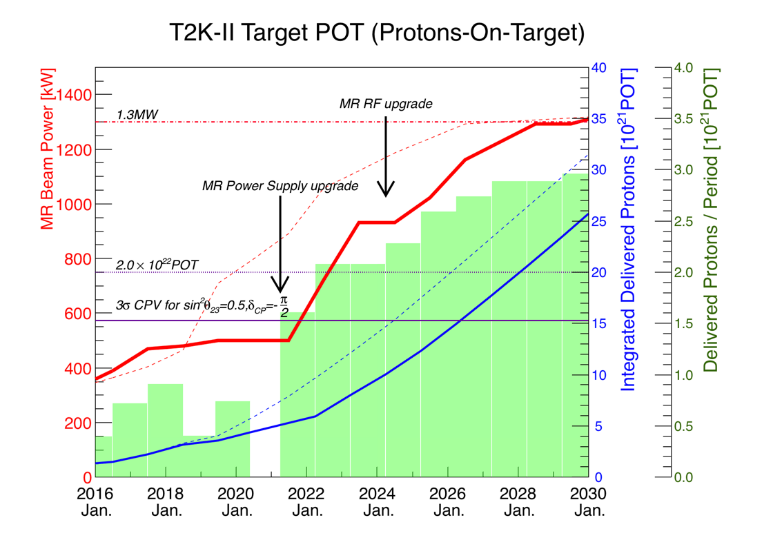
\includegraphics[width=0.6\linewidth]{beam_plan}
  \caption{Target J-PARC beam power (red) and the expected total accumulated statistics (blue) as a function of the year. Two possible schedules are considered shown with solid and dashed lines.}
  \label{fig:up:beam_plan}
\end{figure}

The beamline power upgrade schedule is shown in \autoref{fig:up:beam_plan}. The accelerator will be stopped for one year for the major hardware improvement. In the following years, the intensity will slightly grow alongside the data collection. The target power 1.3 MW is planned to be reached by 2028. This is beyond T2K. The Hyper-Kamiokande experiment is going to use the same beamline and use all the benefits from the power upgrade after the T2K. The details about the beamline upgrade are widely described in~\cite{Abe2019h}.

\section{Detector overview}
\label{sec:up:nd}


\subsection{Current detector limitations}
The T2K off-axis near detector is widely described in \autoref{sec:T2K:nd280} of \autoref{ch:T2K:general}. The schematic view of the setup is presented in \autoref{fig:T2K:ND280} (b). There are several known problems that limit the performance of the ND280. As a result, the total T2K systematics is dominated by the neutrino cross-section and flux uncertainty. These uncertainties could be reduced with better constraints with the upgraded ND280.

One of the main issues is limited phase-space coverage. An event display of a neutrino interaction in the ND280 as well as the detector layout is shown in \autoref{fig:up:ed_fgd1}. The scintillator neutrino targets (Fine Grained Detectors) are shown in violet. They are alternated with 3 TPCs shown in blue. Such a setup is perfect for the reconstruction of the forward and backward going particles. But if the lepton from the neutrino interaction goes at a high angle w.r.t. the beam (up/down in \autoref{fig:up:ed_fgd1}) we will not be able to perform accurate measurements. It will not leave a long enough track in the TPCs, hence we could not estimate the momentum with the curvature and the particle type with the energy loss. It is even possible that the particle goes alone the single vertical bar in FGD. In this case, even tracking with the scintillator detector is impossible. The efficiency of the muon selection from the $\nu_\mu CC$ interactions in the FGD1 over the outgoing lepton angle is shown in \autoref{fig:up:cos_eff_current}.

The far detector can detect the outgoing lepton with uniform efficiency over the 4$\pi$ phase-space. But the near detector could measure only neutrino interactions producing forward going leptons. The comparison of the detectors' acceptance and the expected lepton phase space are shown in \autoref{fig:up:ps}. To extend the constraints from the ND280 to the full phase-space various models of the neutrino interactions are used. But the uncertainties of such models are quite high. The direct measurements of the leptons in 4$\pi$ angle in the near detector will dramatically reduce the systematic uncertainty.

\begin{figure}[!ht]
  \centering
  \begin{minipage}{0.49\linewidth}
      \begin{flushleft}
      \begin{minipage}{0.9\linewidth}
      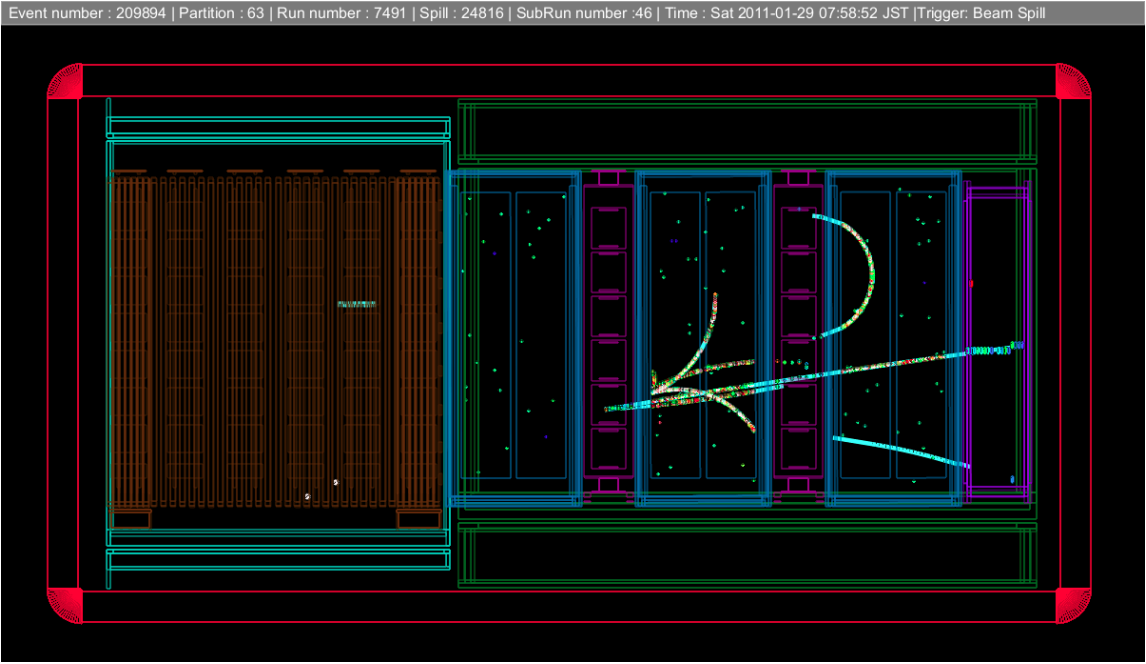
\includegraphics[width=\linewidth]{ed_fgd1}
      \caption{The event display of the neutrino interaction in the FGD1 in the ND280. The beam is coming from the left.}
      \label{fig:up:ed_fgd1}
      \end{minipage}
      \begin{minipage}{0.1\linewidth}
      \end{minipage}
      \end{flushleft}
  \end{minipage}
  \begin{minipage}{0.49\linewidth}
      \begin{flushright}
      \begin{minipage}{0.1\linewidth}
      \end{minipage}
      \begin{minipage}{0.9\linewidth}
      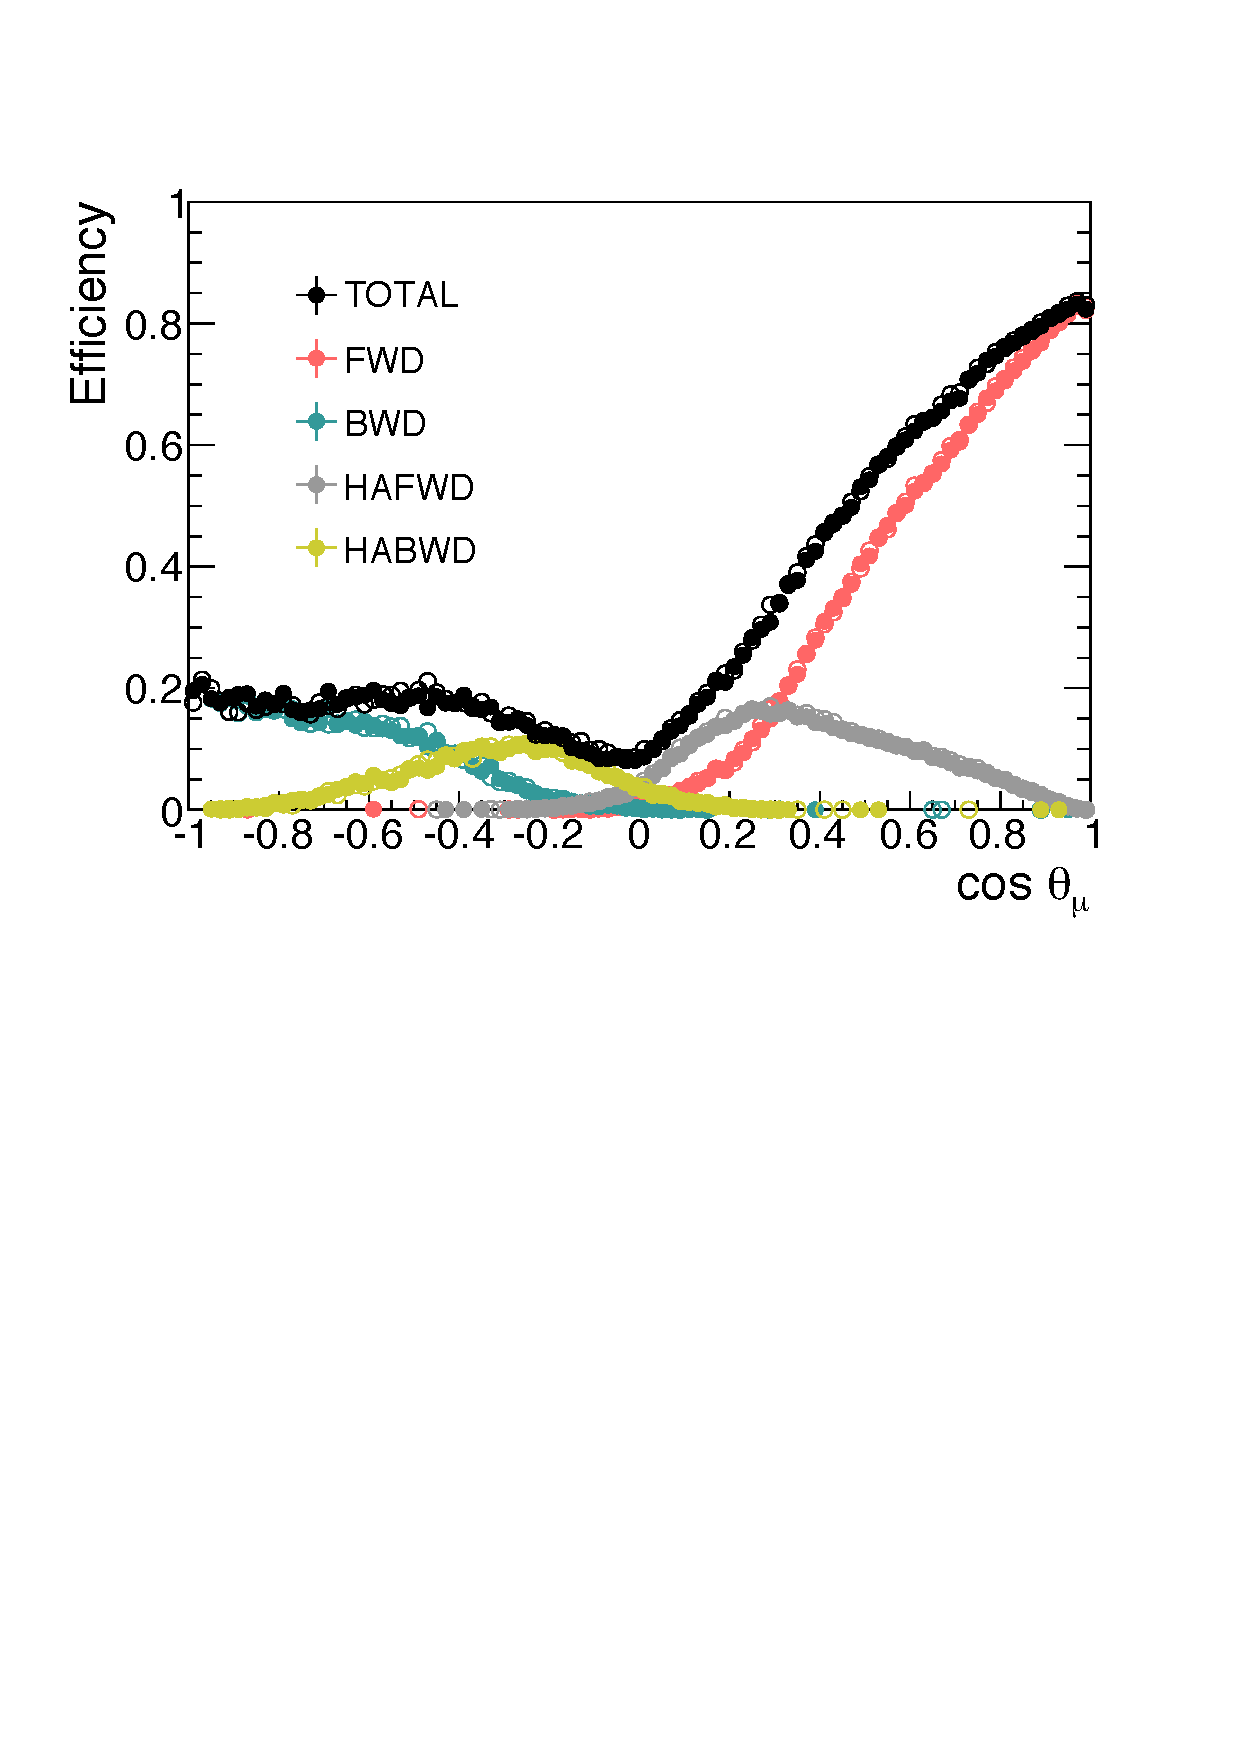
\includegraphics[width=\linewidth]{cos_eff_current}
      \caption{Muon selection efficiency from the $\nu_\mu CC$ interactions in the FGD1 as a function of the lepton angle w.r.t. Z axis.}
      \label{fig:up:cos_eff_current}
      \end{minipage}
      \end{flushright}
  \end{minipage}
\end{figure}

\begin{figure}[!ht]
  \centering
  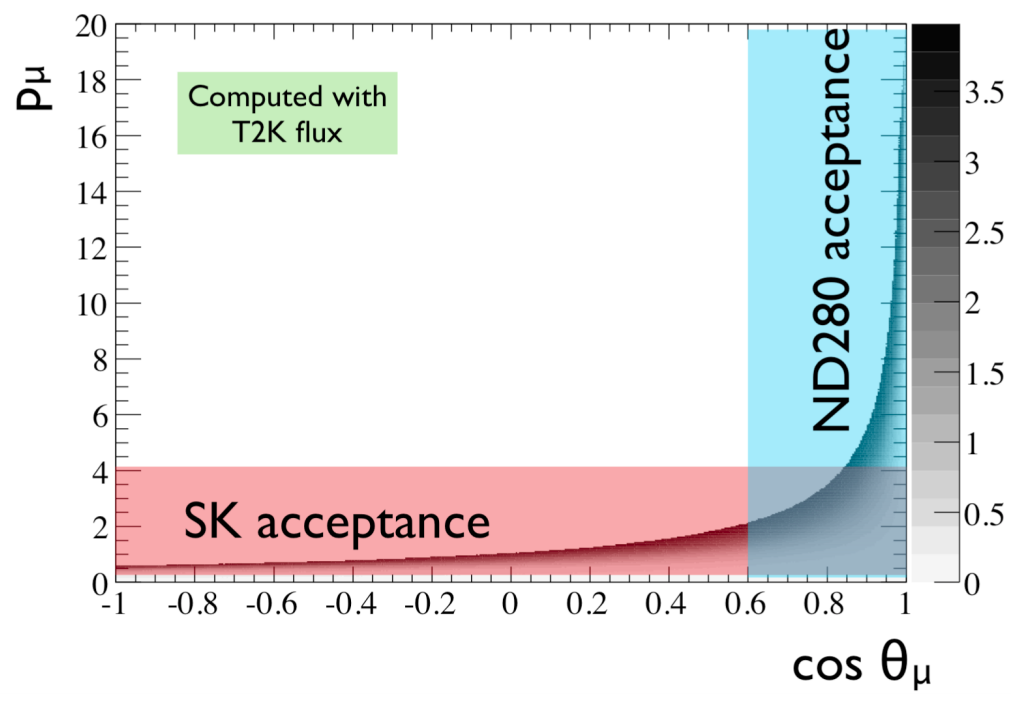
\includegraphics[width=0.5\linewidth]{nd_sk}
  \caption{The acceptance of both near and far detectors of the T2K experiment over the expected lepton phase space.}
  \label{fig:up:ps}
\end{figure}


The other subject of concern is the threshold of particle detection. Thanks to muon penetration ability, they are leaving a long track and could be easily detected. But protons from the neutrino interactions are mostly low energetic and travel a short distance. It's quite difficult to detect them with the sandwich scintillator detector like FGD. The proton should go through at least a few layers for robust detection. If it is pointing at a high angle w.r.t. beam the situation is even worse. The current threshold of the proton detection in FGDs is around 500 MeV, while the proton spectrum starts from 200 MeV. Nucleon detection from the neutrino interaction is extremely important in the T2K. As mentioned in \autoref{ch:T2K:general}, Super--Kamiokande uses CCQE interaction assumption to reconstruct the neutrino energy. But in most of the cases, neutrino doesn't interact with the free nucleon but with Oxygen nuclei in SK and with Carbon and Oxygen nuclei in ND280. The nuclear effects (\autoref{sec:intro:nuclei} of \autoref{ch:nu_phys}) are biasing the neutrino energy measurements. They could even change the event topology. For example, after neutrino interacts with pion production, the pion could be absorbed in the nuclei and the event will look like the CCQE interaction. That's why nuclear effects should be precisely constrained. It could be done with the precise measurement of both outgoing lepton and nucleon kinematics. The detection of short pion tracks will also help with the proper reconstruction of the interaction topology and will gain the neutrino energy estimation accuracy as well.

\subsection{New design proposal}

To improve the performance of the near detector its upgrade was proposed~\cite{Abe2019}. The ND280 tracker (2 FGDs and 3 TPCs) will be kept in place and will continue operation. Thus the data from both T2K-I and T2K-II could be analyzed together. The $\pi^0$ detector will be replaced with the new neutrino target and 2 horizontal TPCs. The upstream part will be surrounded by the time of flight (ToF) detectors. The various CAD models are presented in \autoref{fig:up:nd_up} and \autoref{fig:up:nd_cad}.

\begin{figure}[!ht]
  \centering
  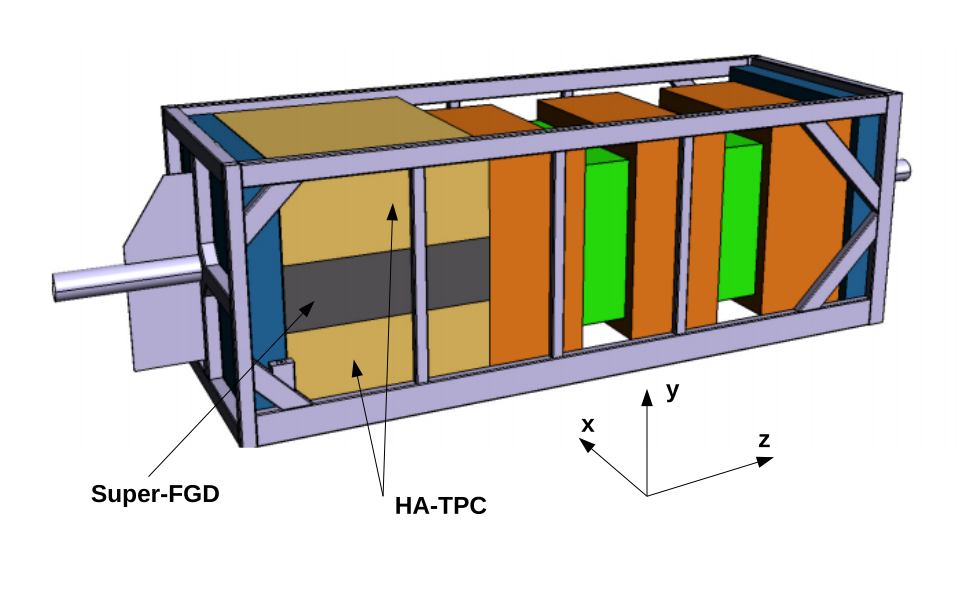
\includegraphics[width=0.5\linewidth]{nd_up}
  \caption{The scheme of the upgraded near detector. The downstream part is kept as it is. The new horizontal target and two high angle TPCs are put in the upstream part,}
  \label{fig:up:nd_up}
\end{figure}

\begin{figure}[!ht]
  \centering
  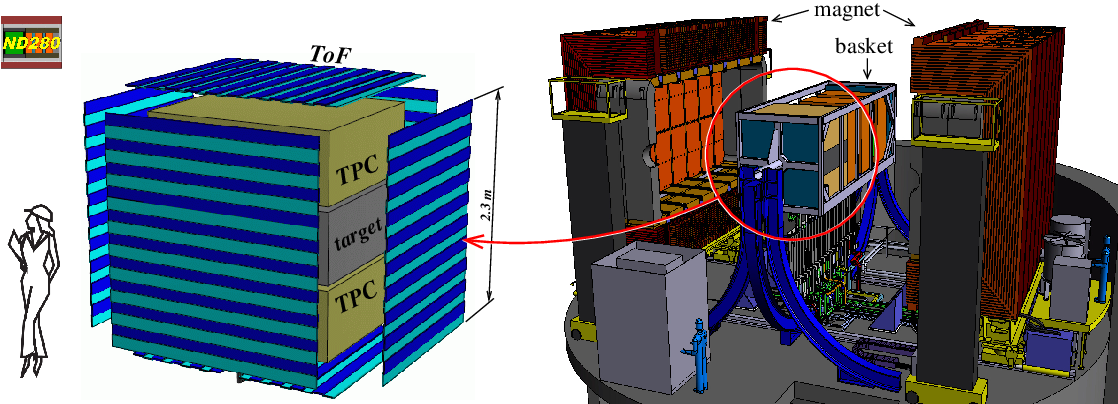
\includegraphics[width=\linewidth]{nd_CAD}
  \caption{The CAD model of the whole upgraded detector setup and the inset of the mostly affected by the modifications upstream part.}
  \label{fig:up:nd_cad}
\end{figure}

The new neutrino target Super-FGD (SFGD) will be composed of small plastic scintillator cubes. The cube edge is set to 1 cm providing fine granularity. Three orthogonal holes are drilled in the cube for the light readout with the WLS fibers. Thus the Super-FGD could reconstruct the tracks in 3D. High granularity significantly reduces the threshold of particle tracking. Also, such a structure will improve the separation between gamma conversion and electron neutrino CC interaction resulting in more precise $\nu_e$ cross-section measurements. The dimensions of the new target are $182\times184\times56 \text{ cm}^3$ giving the total mass close to 2 tonnes. The total fiducial mass of the ND280 will be nearly doubled. The large size of the target allows detecting the secondary interactions of the neutrons from the anti-neutrino CCQE interactions $\overline{\nu}+p\to\ell+n$. As mentioned in the \nameref{ch:up:motif} measurement of the outgoing nucleons are critical for the precise neutrino energy reconstruction and probing neutrino interactions models. The details of the neutron detection proposal are presented in \autoref{ch:up:neutron}. More details about SFGD detector will be provided in \autoref{ch:up:sfgd}.

Two atmospheric pressure High angle TPCs (HATPC) will be put above and below Super-FGD. They will enlarge the phase space to the full coverage. The readout will be organized by the micromegas as for the current TPC, but new technology will be implemented. The detectors will be covered with the resistive foil resulting in the charge spreading over the pads. Thus the spatial resolution could be improved with the same pad size. It will lead to better momentum reconstruction and finally more accurate neutrino energy estimations. The details about HATPC detector will be provided in \autoref{ch:up:tpc}.

The Time of Flight (ToF) detectors will fully cover the upstream part of the ND280. It will be composed of scintillator bars and readout with the MPPC arrays. This detector will help with the reconstruction of the particle direction: to/from Super-FGD. Neutrino interacts quite often in the magnet coil and ECal and could produce a particle that will stop inside the SFGD. The relatively short track inside the scintillator target is not sufficient for the direction reconstruction, but the ToF detectors will give a clear answer. Also, this detector could help with particle identification. For example positrons and protons have very similar dE/dx around 1 GeV/c and could not be distinguished with the TPC but the time of flight is dramatically different.

To sum up, the upgraded ND280 will have several benefits comparing to the present setup:
\begin{itemize}
  \item full phase space coverage for the particles produced in neutrino interactions
  \item low threshold of the particle detection
  \item doubled fiducial mass
  \item better separation of the particles going "in" and "out" the target
  \item electron/gamma separation, resulting in better $\nu_e$ measurements
  \item neutron detection from $\overline{\nu}$ interactions
\end{itemize}

\section{Simulations}
\label{ch:up:sim}

Different configurations mu and ele selection



\chapter{Time Projections Chambers (TPC)}
\label{ch:up:tpc}
The combination of the TPCs and scintillator detectors in ND280 provides accurate physics measurements of the neutrino interactions. The precision of the oscillation analysis is gained a lot with the data collected with the near detector. The TPCs play a key role in the reconstruction of daughter particles from neutrino interactions. The momentum and charge are reconstructed with the track curvature, the particle type is estimated with the ionization energy loss (dE/dx). During the ND280 upgrade, two new TPC will be placed above and below the scintillator target and will be aimed for high angle track detection. Therefore the new detectors are called High--Angle TPC (HA--TPC). It is critical to meet the requirements of the existing TPCs and to study the possibilities of improvements. The momentum resolution of the current TPCs is ~10\% at the momentum around 1 GeV/c. It was driven by the accuracy of the neutrino energy reconstruction. The quasi--elastic reaction is assumed to compute the neutrino energy. In this assumption an initial nucleon stays in rest and is free. We are studying neutrino interactions with the nuclei where nucleons don't satisfy these conditions. Thus the reconstructed neutrino energy will be smeared because of nuclear effects. Fermi motion will be the dominating smearing effect. In the Oxygen and Carbon nucleon movement is characterized with the Fermi momentum $p_F\approx 200$ MeV/c. It will give ~10\% uncertainty for the neutrino energy measurements. With the HA--TPCs, we are going to measure tracks with high angle w.r.t. the beam thus with lower momentum. Lower momentum will result in the larger track curvature and more precise reconstruction. Hence the same spatial resolution as in the current TPC is the minimum requirement for the new detectors, but there will be also no physics benefits from the dramatical spatial resolution improvement. We are going to use the resistive Micromegas technology (\autoref{sec:up:nd}) that will allow making the pads larger, but keep the spatial resolution unchanged or even slightly improve it. The spatial resolution of the current TPCs is at the level of 800 $\mu\text{m}$.

The other critical point for the ND280 performance is the dead material between subdetectors. The TPCs provide excellent tracking for the charged particles so it's strongly desired to detect all the particles that exit the scintillator towards the TPCs with minimal distortions. In the case of a massive field cage or a high Z material, several particles will lose the energy and suffer from multiple scattering making the precise measurements impossible. In the new TPCs, we are going to use a field cage made of a solid insulator laminated on a composite material. Thus the dead material between the scintillator target and the HA-TPC will be minimized. It's an important improvement as high--angle tracks are low energetic and even a small amount of material could cause track distortions. Also, the new field cage will maximize the fiducial volume of the detector.

A good energy resolution is essential for separation electrons and muons. As we are going to measure $\nu_e$ cross--sections while the $\nu_e$ contamination in the neutrino beam is at the level of 1\% the superior $e/\mu$ separation in the TPC is required. The current TPCs provide an 8\% energy resolution that results in 4$\sigma$ separation between electron and muon. The performance of the new detectors should be at least at the same level.

\section{Concept}
The schematic view of the HA--TPC is presented in Figure~\ref{fig:up:tpc_s} and the main parameters are listed in \autoref{tbl:up:tpc_p}. The TPC will consist of a rectangular box divided into 2 parts with the high voltage cathode. The box serves as a gas vessel and a field cage. The field cage provides a uniform electric field inside the box. The high field uniformity is necessary for the uniform electron drift velocity. The latter is essential for the precise measurements of the track position along the drift distance. The signal from the drift electrons is amplified and read-out with the 16 Micromegas modules, 8 at each side. The analog electrical signal is digitized with Front--End Cards (FEC), processed with Front--End Mezzanine cards (offset correction, zero-suppression, etc.), and then transferred to the ND280 global data acquisition system. The FEM and FEM cards are mounted on the TPC itself. The signal acquisition scheme is similar to the one we use in the existing TPCs.

\begin{table}
\begin{minipage}[!ht]{0.49\linewidth}
  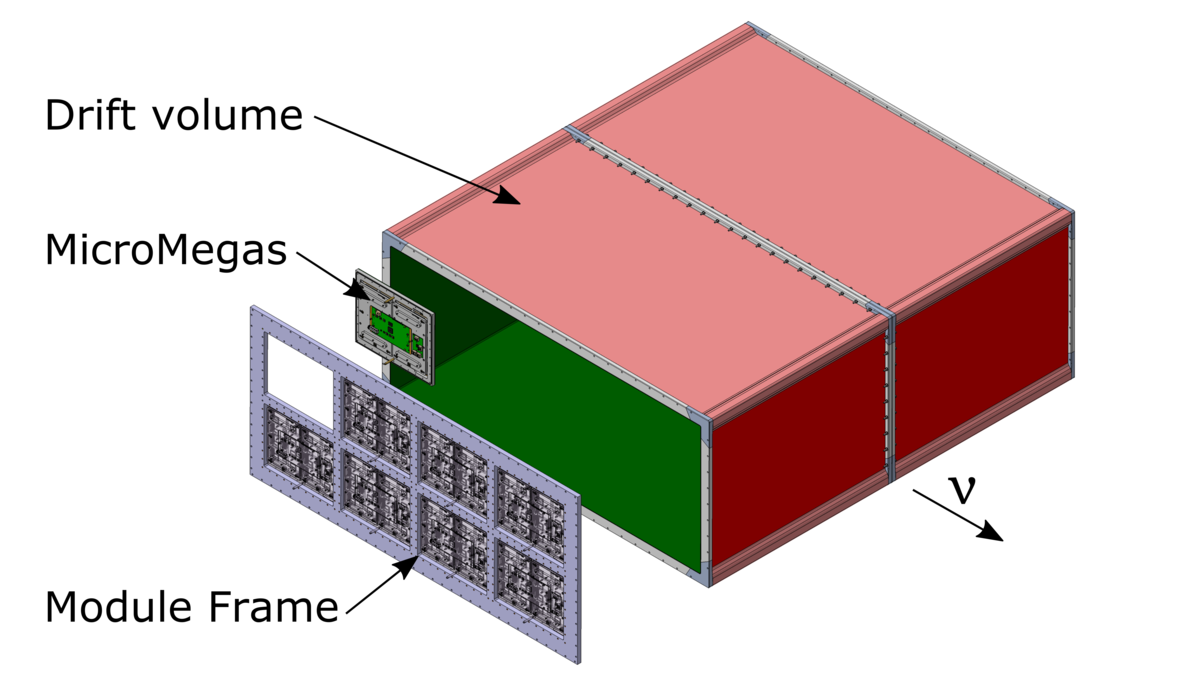
\includegraphics[width=\linewidth]{HATPC_scheme}
  \captionof{figure}{The schematic view of the new TPC}
  \label{fig:up:tpc_s}
\end{minipage}
\hfill
\begin{minipage}[!ht]{0.49\linewidth}
  \begin{tabular}{|c|c|}
    \hline
    Parameter             & Value \\
    \hline
    Overall x$\times$y$\times$z (m)   & 2.0$\times$0.8$\times$1.8 \\
    Drift distance (cm)               & 90 \\
    Magnetic Field (T)                & 0.2 \\
    Electric field (V/cm)             & 275 \\
    Gas Ar-CF4-iC4H10 (\%)            & 95-3-17 \\
    Drift Velocity cm/$\mu$s          & 7.8 \\
    Transverse diffusion ($\mu$m/$\sqrt{\text{cm}}$) & 265 \\
    Micromegas gain                   & 1000 \\
    Micromegas dim. z$\times$y (mm)   & 340$\times$410 \\
    Pad z$\times$y (mm) & 10$\times$11 \\
    N pads                            & 36864 \\
    el. noise (ENC)                   & 800 \\
    S/N                               & 100 \\
    Sampling frequency (MHz)          & 25 \\
    N time samples                    & 511 \\
    \hline
  \end{tabular}
  \caption{Main parameters of the new TPC}
  \label{tbl:up:tpc_p}
\end{minipage}
\end{table}

The requirements set for the field cage are to contain as little material as possible and use only low Z elements to minimize a photon conversion and a charged particle scattering. At the same time, the box should be tight enough to hold the gas pressure without leakage, prevent atmospheric Oxygen and Nitrogen from entering the box, and contaminating the gas mixture. The walls of the field cage should be flat to prevent a high voltage discharge. To meet the requirements mentioned above the composite material was chosen for the cage box. The composite materials are widely used in the industry. The TPC wall is going to be consist of an Aramid honeycomb core and laminate skins on both sides of the core. In the inner part, the box will be covered with Kapton foil covered by Copper strips. It the main field forming element of the structure.

The total thickness of the new field cage is 30 mm and its ratio to the radiation length is $d/X_0=1.7$. This value is improved comparing to the existing TPC. The old setup consists of two nested boxes 14 and 12 mm thick separated with a 68 mm gap. Also, heavier materials were used. The new structure minimizes the dead space between the HA--TPCs and scintillator targets by three times and suppress the particle track distortions.

\subsection{Resistive MicroMegas technology}
\label{sec:up:res}
The resistive bulk Micromegas technology is going to be used as a readout detector of the HA--TPCs. The TPC working principle is described in \autoref{sec:t2k:tpc} of \autoref{ch:T2K:general}. In short, the drift electrons are amplified with the high electric field between the micro--mesh and readout pads (\autoref{fig:up:res} left). The analog electrical signal is formed in the pads and further transported to the readout electronics. The bulk Micromegas~\cite{Giomataris2005} was proved to have excellent performance and long life--time in the existing experiments. This technology minimizes the dead space on the detector plane and provide an excellent gain uniformity over the whole detector area. They have been operated in the experiments for a long period and the aging effect was found negligible.

\begin{figure}[!ht]
  \centering
  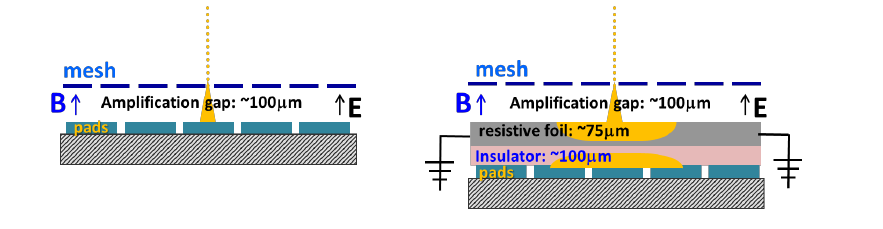
\includegraphics[width=0.8\linewidth]{mm-res}
  \caption{The schematic view of the bulk Micromegas operation without the resistive foil (left) and with resistive foil (right). The charge spreading because of the resistive foil is illustrated.}
  \label{fig:up:res}
\end{figure}

The resistive Micromegas are the upgrade for the existing technology. The pads are covered with an insulator layer and a resistive foil (\autoref{fig:up:res} right). The foil is made of the Kapton layer covered with a thin Diamond-Like-Carbon structure (DLC). Such a design provides natural avalanche quenching. Thus the Micromegas discharge is prevented and there is no need in the protection diodes in the front--end electronics. The resistive layer serves as a two dimensional RC network spreading the charge over the pads. For a point-like charge source the charge density versus the time $t$ and radius $r$ is described with the exponential law:
\begin{equation}
\rho(r,t)=\frac{RC}{2t}e^{-2r^2RC/\left(4t\right)}
\end{equation}

where $R$ and $C$ are resistivity and capacitance for unit area respectively. For example, giving the shaping time equal to 100 ns, resistivity equal to 400 $\text{k}\Omega/\text{mm}^2$, and glue thickness set to 75 $\mu\text{m}$ (controlling the capacity) standard deviation of the charge spreading is expected to be 2.6 mm. Thus the spreading could be controlled with both resistivity and capacity. For example, for the more dramatic spreading, the resistivity could be decreased or/and the thicker glue layer could be used (smaller capacity).

The effect of the charge spreading could improve the spatial resolution of the setup. E.g. the electron cloud is pointed to the pad center and is smaller than the pad size. In the absence of the resistive foil, only one pad will register the signal. In such a case the spatial resolution will be limited by the pad size. While with the charge spreading all the neighbor pads will register some signal. Even a simple barycenter measurement~\cite{Dixit2004} could improve the spatial resolution comparing to the traditional Micromegas. This improvement is the most significant at small drift distances when the electron cloud is compact and not yet expended with the transfer diffusion. In the ND280 TPCs, we observed a dramatic degradation of the resolution for the drift distances smaller than 200 mm because of this effect. The spectacular spatial resolution improvement down to 70 $\mu\text{m}$ with the resistive Micromegas was found for the International Linear Collider (ILC) TPC prototype~\cite{Attie2011}. For the case of the T2K, the resistive Micromegas allow using larger pads without any degradation of the detector performance.

\section{Prototype tests}
The better spatial resolution is going to be achieved with the new TPC with resistive anode. At the same moment, the energy resolution should not decrease as it's critical for the T2K $\nu_e$ measurements. Few detector prototypes were built and tested. The main goals of the tests are to test the detector production technology, to find the most optimal hardware parameters and to estimate the spatial and energy resolution of the future detector.

\subsection{Cosmic test}
\label{sec:up:saclay}
The first test of the T2K TPC module prototype  was done with the test bench in Saclay. The scheme and the photo of the setup are shown in \autoref{fig:tpc:photo_saclay}.

\begin{figure}
  \begin{minipage}{0,33\linewidth}
    \centering
    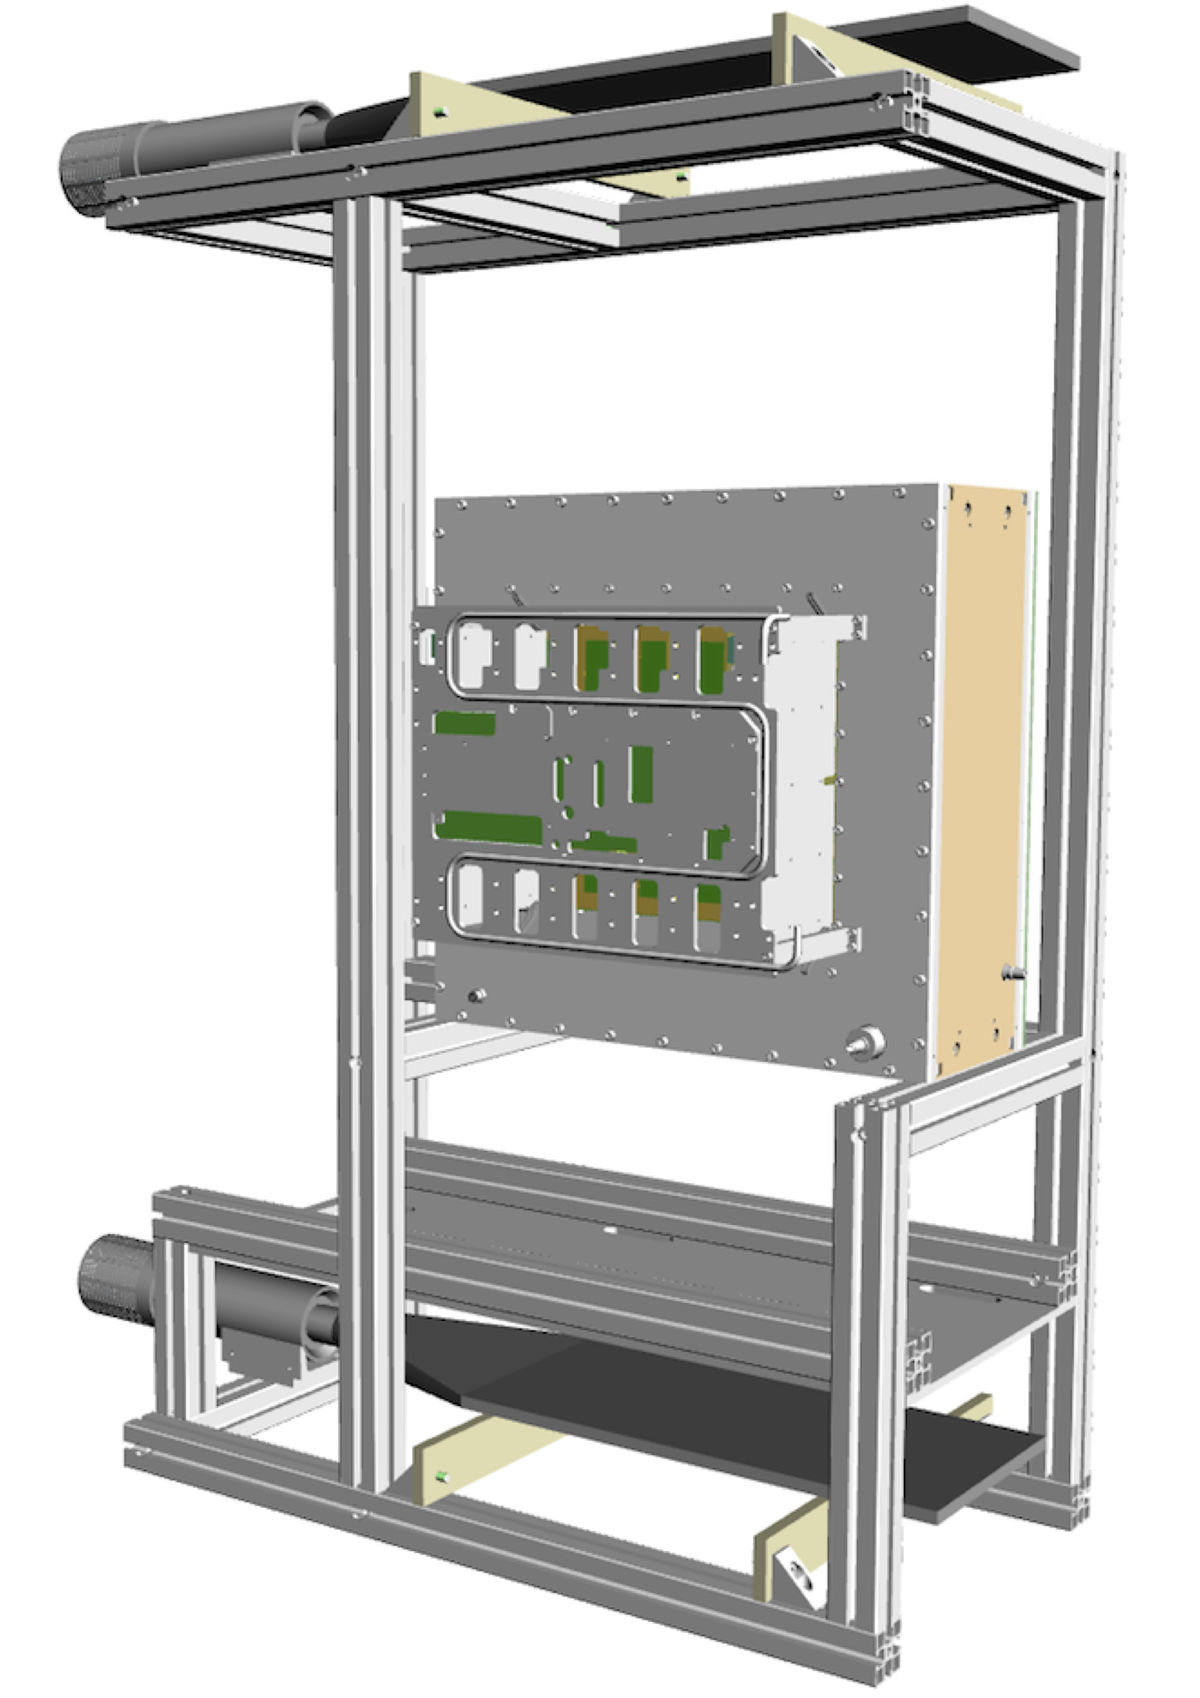
\includegraphics[width=0.5\linewidth]{Saclay_test_bench} \\ (a)
  \end{minipage}
  \begin{minipage}{0,33\linewidth}
    \centering
    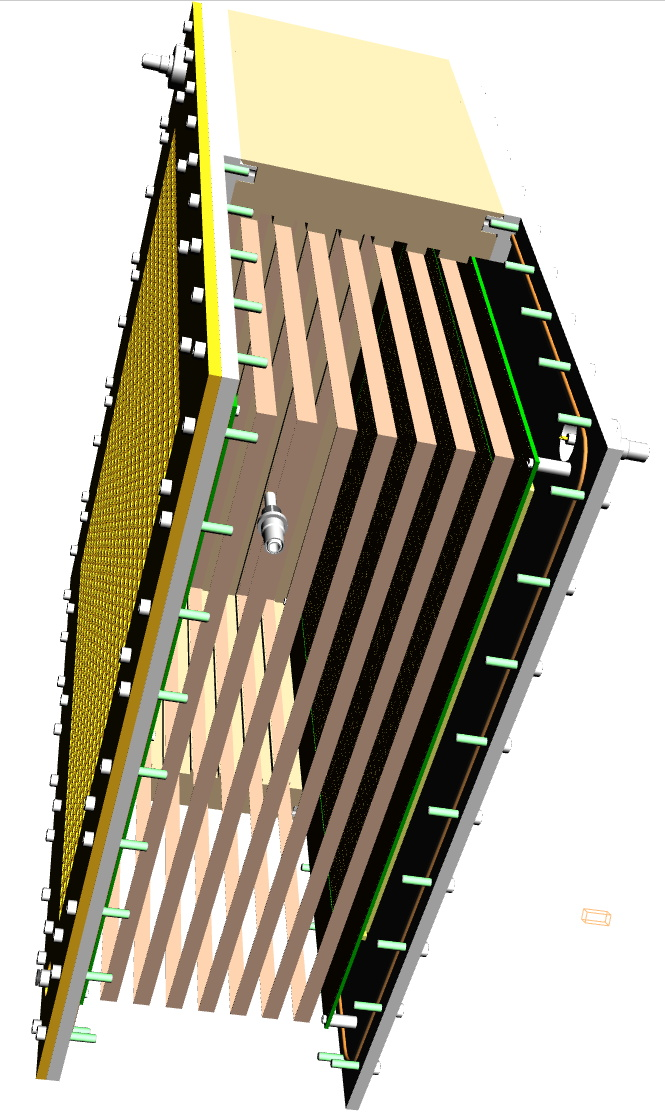
\includegraphics[width=0.5\linewidth]{testbenchTPC} \\ (b)
  \end{minipage}
  \begin{minipage}{0.33\linewidth}
    \centering
    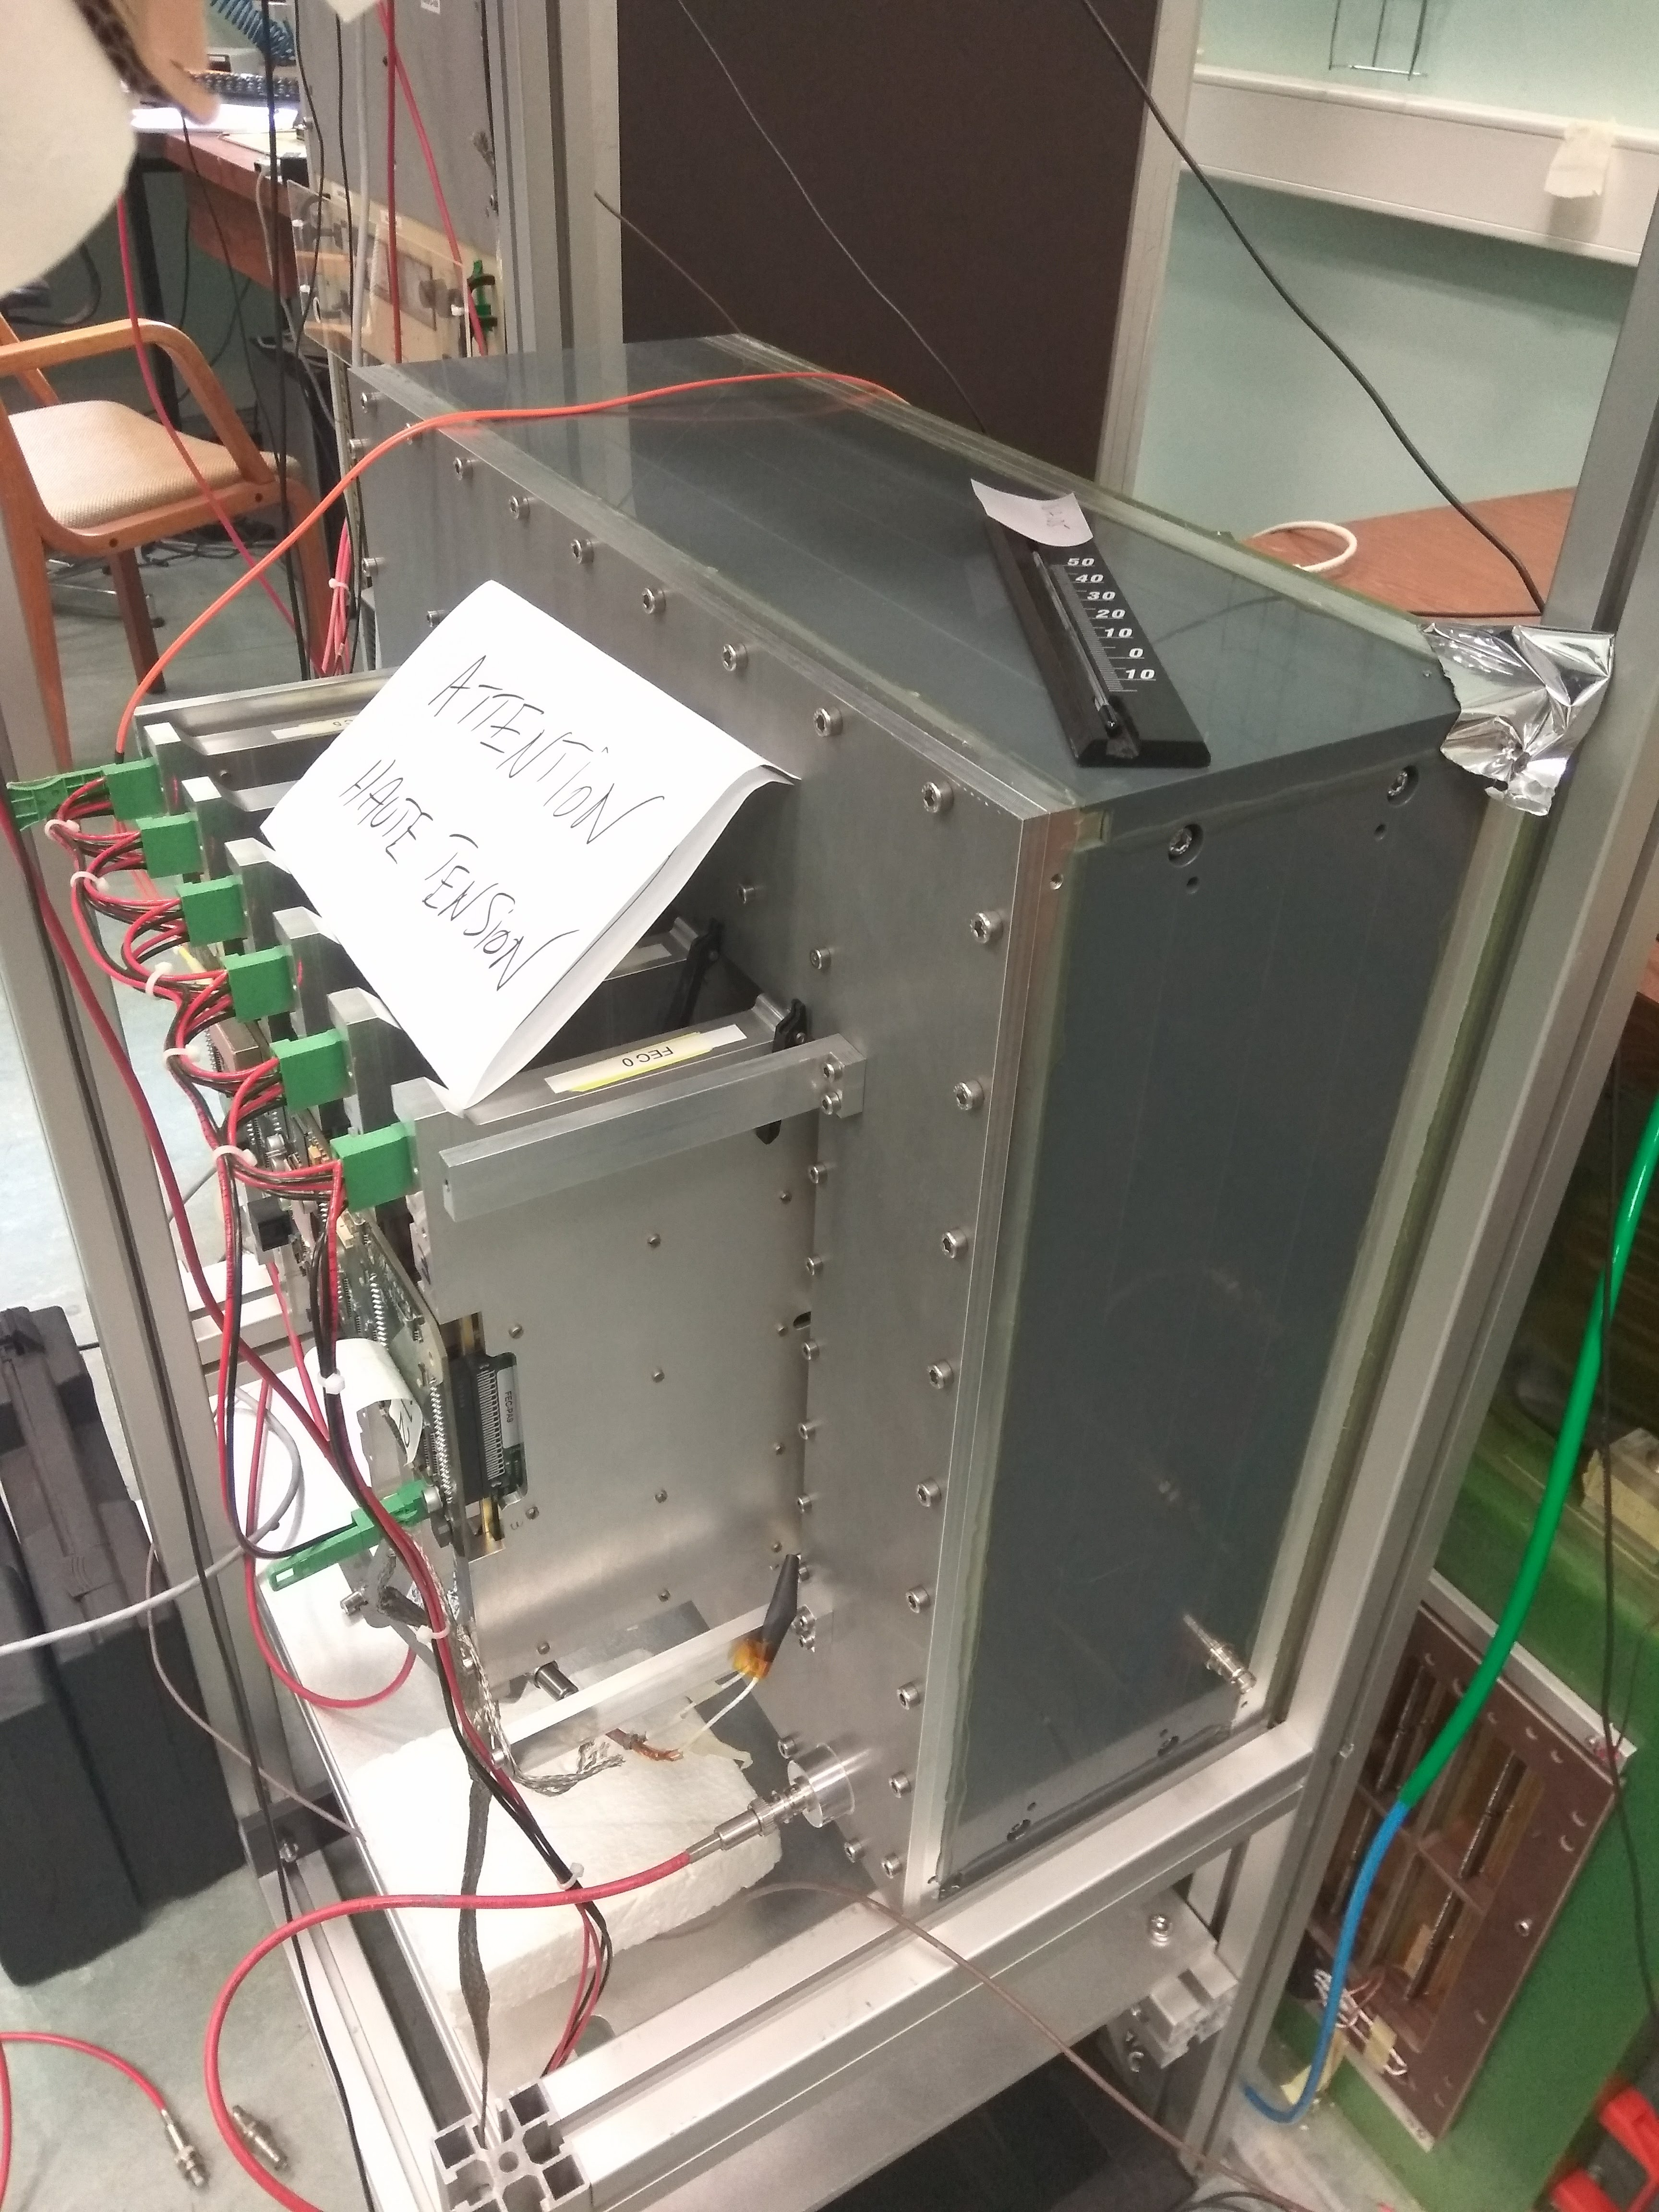
\includegraphics[width=0.5\linewidth]{tpc_saclay_ph} \\ (c)
  \end{minipage}
  \caption{TPC test bench in Saclay. (a) a CAD model of the whole test bench with the scintillator bars above and behind the detector as a trigger. (b) the CAD model of the field cage. (c) a photo of the test bench during the data taking.}
  \label{fig:tpc:photo_saclay}
\end{figure}

The field cage with 15 cm drift region was used for the test setup. It was field with Argon (95\%) and Isobutane(5\%). The uniform electric field is maintained with the strips that you can see on \autoref{fig:tpc:photo_saclay} (b). The drift field is set to 183 V/cm. The resistive Micromegas are mounted on the side of the field cage. The size of the module is 36$\times$34 $\text{cm}^2$ and it is fpaved with 36$\times$48 pads 0.98$\times$0.70 $\text{cm}^2$ each. The RC feature is implemented with 200 $\mu\text{m}$ insulator layer (capacitance) and 50 $\mu\text{m}$ Kapton with a thin Diamond-Like-Carbon layer (DLC) (resistivity). The resistivity value was set to 2.5 MOhm/$\text{mm}^2$. The front--end electronics is mounted on the outer side of the micromegas and could be seen on \autoref{fig:tpc:photo_saclay} (c).

The data was taking with the cosmic rays and the X--ray radioactive source (${}^{55}\text{Fe}$). The trigger system for the cosmic muons was built around the setup. On the \autoref{fig:tpc:photo_saclay} (a) two scintillator planes above and below the detector are shown in dark gray. The planes are readout with photomultipliers and the coincidence of signal in two planes serves as a trigger for the through-going cosmic ray. From the ${}^{55}\text{Fe}$ source we expect the continuous decays, so we could sample the data nearly at any time.The pulse generator was used as a trigger for this sample.

As at any other detector, we expected to see a certain level of noise in our measurements. The noise level was measured for each channel independently. The pulse generator was used to sample the data from each pad. As we expected no signal in the pad the measured value should be caused by the noise and suppressed in the future measurements. As the noise is a subject of fluctuation its value was measured for a continuous period. The measured values were fit with the Gaussian distribution and the mean and sigma characteristics were extracted from the fit. The mean value was going to be subtracted from every measurements done with this particular pad. The sigma value was used to treat the measured amplitude as a signal or a noise. If the amplitude was different from the mean value by more then four sigmas the measurement would be recorded. The procedure described above is called ``zero--suppression''. It is usually quantified with the value of standard deviations used to divide signal and noise, e.g. $4\sigma$ or $5\sigma$ zero--suppression.

The primary goal of the detector test was to figure out that the whole detector plane was operating as expected, the detector response in uniform and the Micromegas were not damaged. The example of the event displays are shown in \autoref{fig:tpc:saclay_ed}. As the gain supposed to be uniform over the whole Micromegas, we expect a uniform measured charge. The hit map obtained with the cosmic rays is shown in \autoref{fig:tpc:hitmap_saclay}.

\begin{figure}[!ht]
  \centering
  \begin{minipage}{0.49\linewidth}
  \centering
    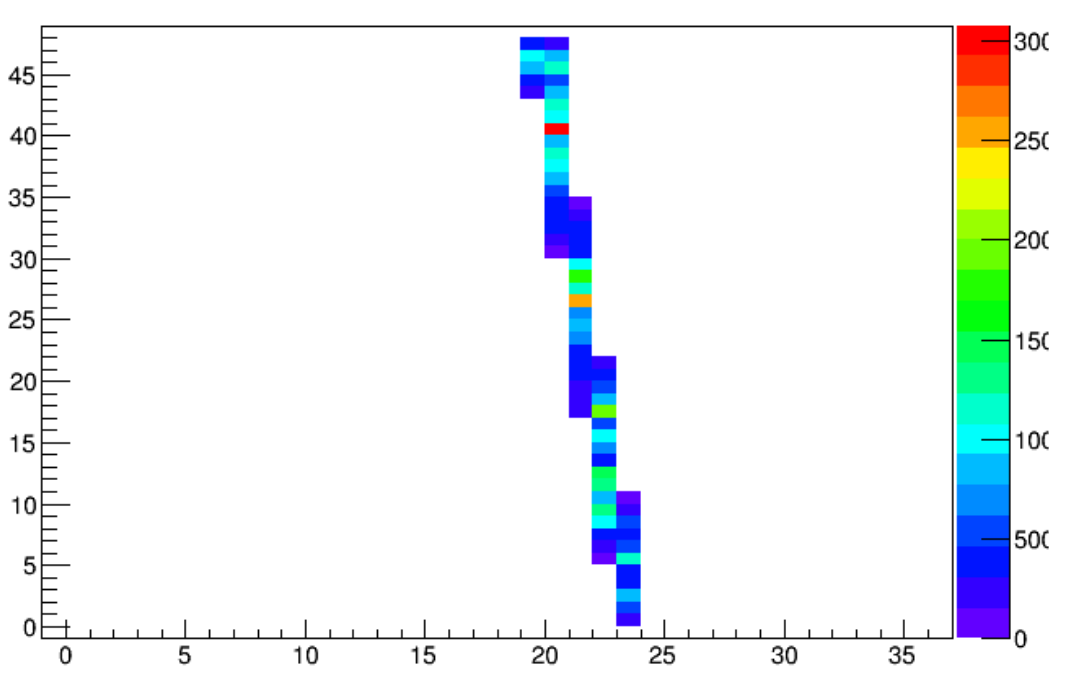
\includegraphics[width=0.8\linewidth]{saclay_track} \\ (a)
  \end{minipage}
  \begin{minipage}{0.49\linewidth}
  \centering
    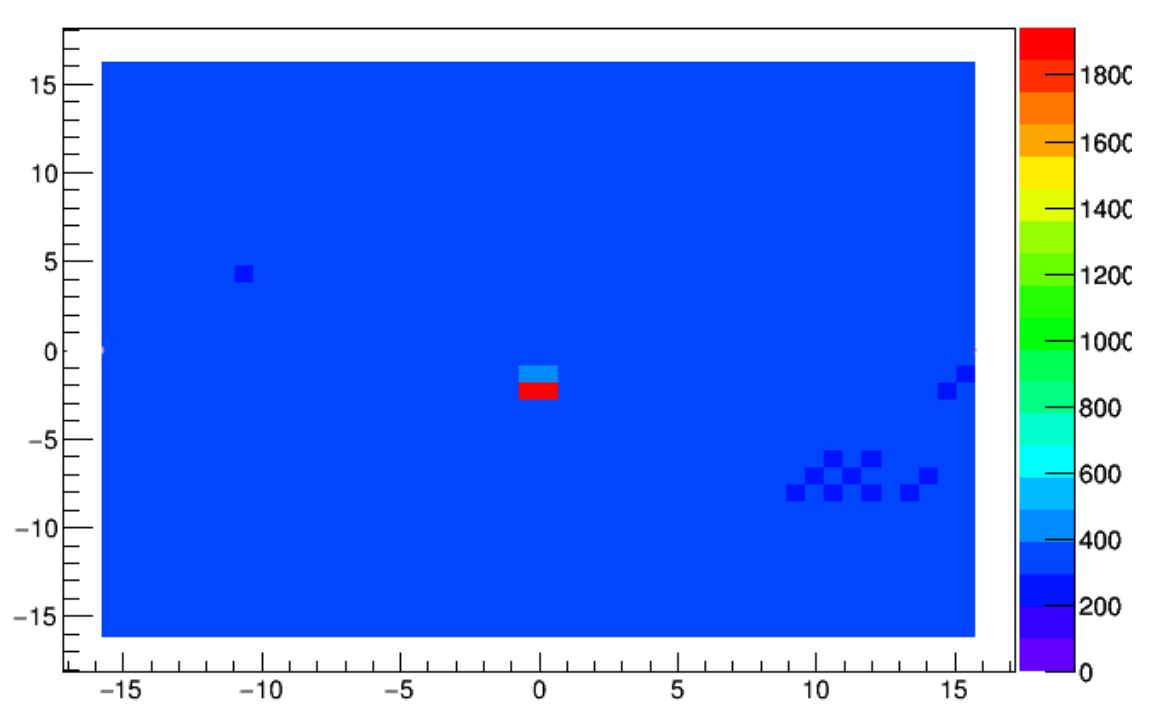
\includegraphics[width=0.8\linewidth]{saclay_source.png} \\ (b)
  \end{minipage}
  \caption{Events observed in the TPC prototype during the test in Saclay. (a) cosmic ray and (b) conversion of the X--ray from ${}^55\text{Fe}$ source.}
  \label{fig:tpc:saclay_ed}
\end{figure}

\begin{figure}[!ht]
  \centering
  \begin{minipage}{0.49\linewidth}
  \centering
    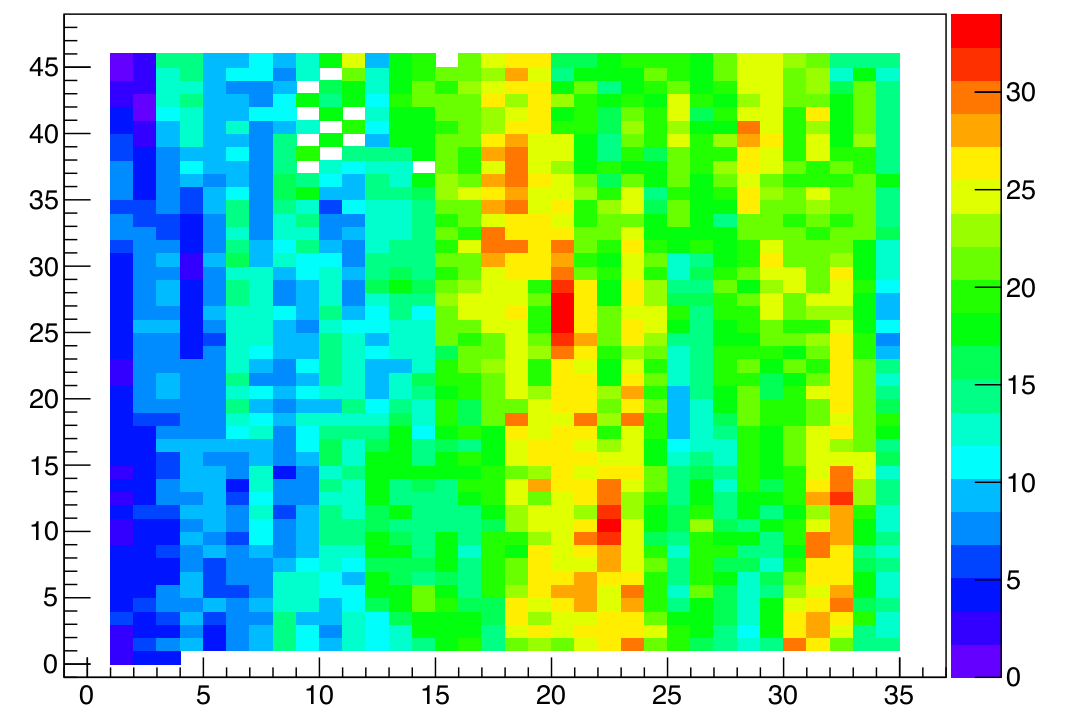
\includegraphics[width=0.8\linewidth]{saclay_hitmap} \\ (a)
  \end{minipage}
  \begin{minipage}{0.49\linewidth}
  \centering
    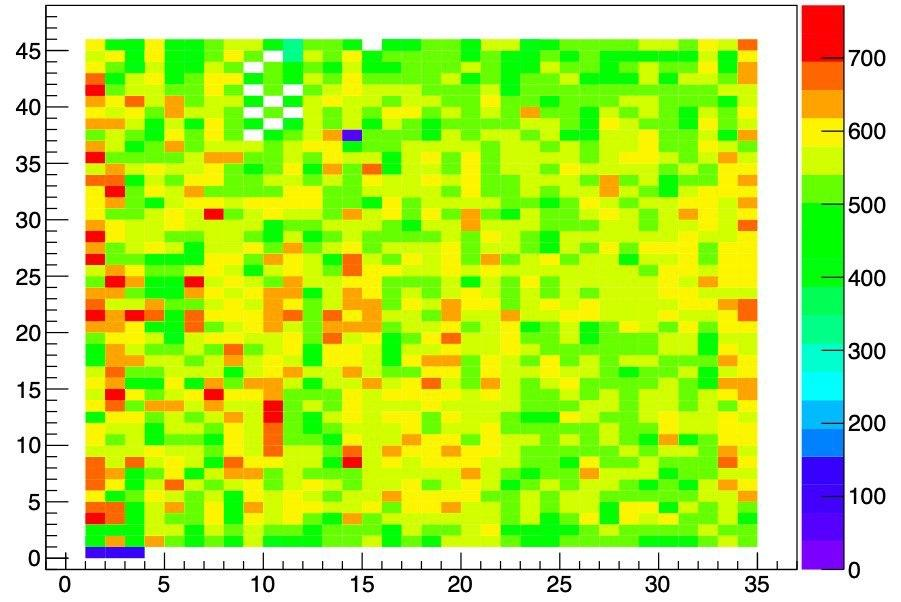
\includegraphics[width=0.8\linewidth]{saclay_hitmap_norm} \\ (b)
  \end{minipage}
  \caption{Hit maps observed in the TPC prototype during the test in Saclay. (a) how many times the particular pad was hit and (b) the average charge measured per a hit.}
  \label{fig:tpc:hitmap_saclay}
\end{figure}

At the hit maps, a cluster of the missed pads was observed at the top left part of the Micromegas. It was found that the problem is in the electronic connection in the readout system, but not in the Micromegas itself.

\subsubsection{TPC energy resolution}
\label{sec:tpc:tpc_dedx}
The energy resolution is critical for the T2K measurements. As mentioned in \autoref{sec:t2k:tpc} of \autoref{ch:T2K:general}, during the ionization process charged particle loose the energy with high fluctuations. The average value of plenty independent measurements is used for the particle type estimations. The resistivity capability implements a correlation of the measured charge values in the neighbor pads. It can spoil the energy resolution as each measurement is not independent anymore. I estimated the energy resolution for the cosmic rays with the Saclay TPC prototype.

First of all the robust tracks should be selected from the sample. I was interested in the vertical tracks that crosses the whole Micromegas. The extremely simple method was developed to obtain the first preliminary results. In ll the events the fit with the straight line is performed. In case of multiple tracks, fit shows the bad quality and the event is skipped. If the fit is successfulness the track position and direction are defined. Only vertical cosmic rays are considered for the analysis. The hits on the both side of the track that have the small time difference w.r.t. the track are assigned to the cosmic ray track. The ``cluster'' is defined as a group of hits in the row, i.e. perpendicular to the track direction. The charge collected in the cluster is sum up and considered as a energy loss per fixed length (0.9 mm --- pad size). The distribution of the charge in the cluster is shown in \autoref{fig:tpc:saclay_charge} (a).

The distribution of the charge per cluster has a long tail towards the high energy. This is in agreement with the expected ionization energy spectrum as it is described with Landau distribution. To omit the clusters with large charge deposition the ``truncation'' method is used. All the clusters in the track are sorted by increasing charge. Some clusters from the beginning of the list (e.g. 70\%) are used to estimate the average energy loss per cluster. The distribution of the ``truncated mean'' of the charge per cluster is shown in \autoref{fig:tpc:saclay_charge} (b). The ionization fluctuations are not affecting the distribution anymore and it is very similar with the Gaussian function. Therefore the mean and the standard deviation could be estimated and then the resolution is computed. This method gives an estimation of the energy resolution at level of 20\%. The resolution is roughly proportional to inverse square root of the track length $\sagma\propto1/\sqrt(l)$. We use only one module 36 cm length, while in the ND280 TPCs are nearly two times longer. The expected resolution of the full-scale resistive detectors is $20/\sqrt(2)\approx14.1\%$. It is higher comparing to the performance of the existing detectors (8\%). But the spectrum of the cosmic rays is not monoenergetic. Thus not only detector smearing but also the initial energy loss will broaden the spectrum. More accurate studies with the charged particles with given momentum will provide more accurate estimations.

\begin{figure}[tb]
  \centering
  \begin{minipage}{0.49\linewidth}
    \centering
    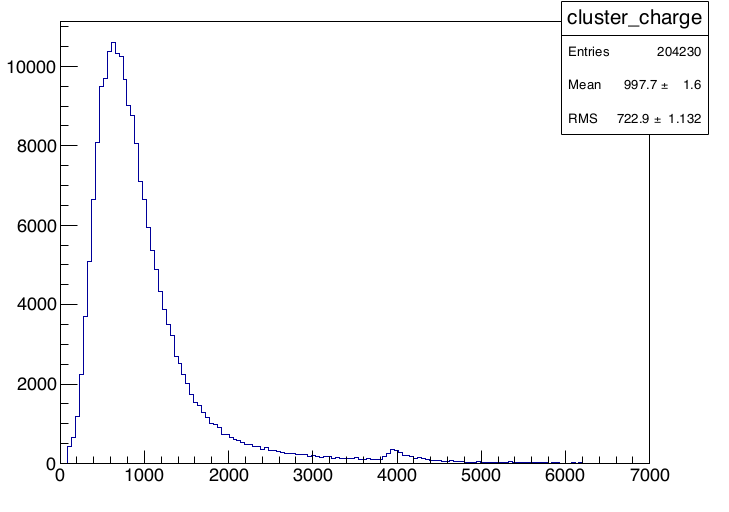
\includegraphics[width=0.8\linewidth]{saclay_charge} \\ (a)
  \end{minipage}
  \begin{minipage}{0.49\linewidth}
    \centering
    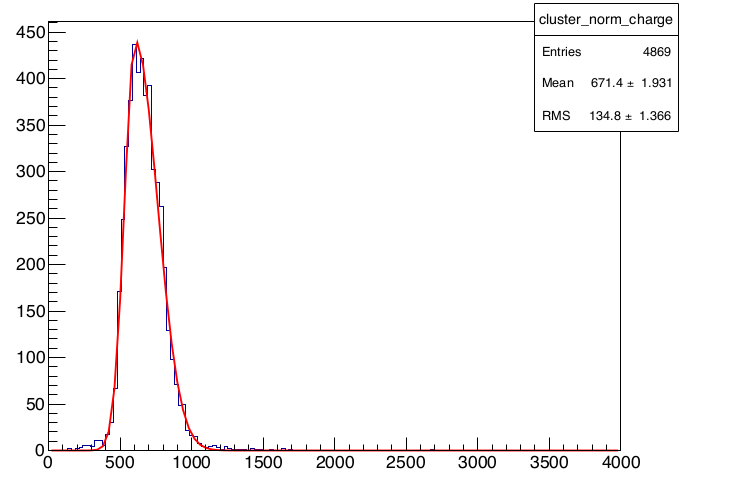
\includegraphics[width=0.8\linewidth]{saclay_trunc} \\ (b)
  \end{minipage}
  \caption{The distribution of the charge in the cluster for the vertical cosmic tracks detected with TPC prototype in Saclay. (a) directly measured charge in each cluster (b) average charge per cluster after the truncation.}
  \label{fig:tpc:saclay_charge}
\end{figure}

\subsubsection{Drift velocity measurements}
\label{sec:tpc:drift}

Above the first preliminary test of the T2K TPC prototype was described. The concept of the charge spreading over pads was proved to be working. The energy resolution was estimated at the level close to one we have in the current ND280 TPCs. Below I will proceed with more detailed analysis to study the detector performance more carefully.

\subsection{CERN beamtest}
The MM from saclay test is used
HARP field cage
energy + drift field.
SR + PRF approach

\subsection{DESY beamtest}


\chapter{Super FGD}
\label{ch:up:sfgd}
\section{Concept}
\subsection{Assembly}
\section{Simulations}
\subsection{Expected light yield}
\subsection{Michell electron tagging}
\subsection{Pileups}
\section{Beamtest}
\subsection{First CERN beamtest}
\subsection{Second CERN beamtest}

\chapter{Neutron tagging in SuperFGD}
\label{ch:up:neutron}
\section{Motivation}
\section{Geant4 simulation}
\section{Efficiency and energy resolution}
\section{Background estimations}
\section{Prospects for physics}
\end{document}